\documentclass[tikz,border=0pt]{standalone}
\usepackage{graphicx}
\usepackage{amsmath,amssymb}
\usepackage{times}

\begin{document}
\begin{tikzpicture}[x=1pt,y=1pt]
  \path[use as bounding box] (0,0) rectangle (399.12,95.28);
  \node[anchor=south west,inner sep=0] at (0,0) {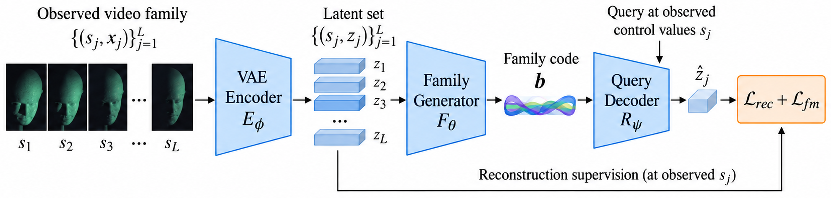
\includegraphics[
    width=399.12pt,height=95.28pt
  ]{figures/source_data/fig2a_codec_training_original.pdf}};

  % Frozen video VAE. The polygon covers the legacy E_phi label exactly.
  \filldraw[
    draw=blue!70!cyan,line width=0.48pt,
    left color=cyan!4,right color=blue!18
  ] (102.95,19.20) -- (140.45,28.55) -- (140.45,67.70) --
    (102.95,77.25) -- cycle;
  \node[align=center] at (121.70,49.20) {\fontsize{7.7}{8.1}\selectfont
    VAE\\[-0.4pt]Encoder\\[-0.2pt]$\mathcal E$\\[-1.2pt]
    {\fontsize{4.3}{4.8}\selectfont (frozen)}};

  % Generic LFVD family encoder shared by Identity, Mix, and Compact.
  \filldraw[
    draw=blue!70!cyan,line width=0.48pt,
    left color=cyan!4,right color=blue!18
  ] (194.75,20.80) -- (233.95,29.90) -- (233.95,66.40) --
    (194.75,76.00) -- cycle;
  \node[align=center] at (214.25,51.10) {\fontsize{7.5}{8.0}\selectfont
    Family\\[-0.3pt]Encoder\\[-0.1pt]$E_\phi$};
  \node[align=center] at (214.25,16.75) {\fontsize{4.15}{4.5}\selectfont
    Identity / Mix / Compact};

  % Codec reconstruction is optimized separately from flow matching.
  \filldraw[
    draw=orange!85!red,line width=0.48pt,rounded corners=2.0pt,
    left color=orange!5,right color=orange!12
  ] (354.00,35.25) rectangle (397.35,58.90);
  \node at (375.65,47.05) {\fontsize{9.2}{9.5}\selectfont
    $\mathcal L_{\mathrm{codec}}$};
\end{tikzpicture}
\end{document}
